\PassOptionsToPackage{unicode=true}{hyperref} % options for packages loaded elsewhere
\PassOptionsToPackage{hyphens}{url}
%
\documentclass[ignorenonframetext,aspectratio=169]{beamer}
\usepackage{pgfpages}
\setbeamertemplate{caption}[numbered]
\setbeamertemplate{caption label separator}{: }
\setbeamercolor{caption name}{fg=normal text.fg}
\beamertemplatenavigationsymbolsempty
% Prevent slide breaks in the middle of a paragraph:
\widowpenalties 1 10000
\raggedbottom
\setbeamertemplate{part page}{
\centering
\begin{beamercolorbox}[sep=16pt,center]{part title}
  \usebeamerfont{part title}\insertpart\par
\end{beamercolorbox}
}
\setbeamerfont{section title}{size=\Huge}
\setbeamertemplate{section page}{
\centering
\begin{beamercolorbox}[sep=12pt,center]{part title}
  \usebeamerfont{section title}\insertsection\par
\end{beamercolorbox}
}
\setbeamertemplate{subsection page}{
\centering
\begin{beamercolorbox}[sep=8pt,center]{part title}
  \usebeamerfont{subsection title}\insertsubsection\par
\end{beamercolorbox}
}
\AtBeginPart{
  \frame{\partpage}
}
\AtBeginSection{
  \ifbibliography
  \else
    \frame{\sectionpage}
  \fi
}
\AtBeginSubsection{
  \frame{\subsectionpage}
}
\usepackage{lmodern}
\usepackage{amssymb,amsmath}
\usepackage{ifxetex,ifluatex}
\usepackage{fixltx2e} % provides \textsubscript
\ifnum 0\ifxetex 1\fi\ifluatex 1\fi=0 % if pdftex
  \usepackage[T1]{fontenc}
  \usepackage[utf8]{inputenc}
  \DeclareUnicodeCharacter{03B5}{$\epsilon$}
  \DeclareUnicodeCharacter{03C3}{$\sigma$}
  \usepackage{textcomp} % provides euro and other symbols
\else % if luatex or xelatex
  \usepackage{unicode-math}
  \defaultfontfeatures{Ligatures=TeX,Scale=MatchLowercase}
\fi
% use upquote if available, for straight quotes in verbatim environments
\IfFileExists{upquote.sty}{\usepackage{upquote}}{}
% use microtype if available
\IfFileExists{microtype.sty}{%
\usepackage[]{microtype}
\UseMicrotypeSet[protrusion]{basicmath} % disable protrusion for tt fonts
}{}
\IfFileExists{parskip.sty}{%
\usepackage{parskip}
}{% else
\setlength{\parindent}{0pt}
\setlength{\parskip}{6pt plus 2pt minus 1pt}
}
\usepackage{hyperref}
\hypersetup{
            pdfborder={0 0 0},
            breaklinks=true}
\urlstyle{same}  % don't use monospace font for urls
\newif\ifbibliography
\usepackage{color}
\usepackage{fancyvrb}
\newcommand{\VerbBar}{|}
\newcommand{\VERB}{\Verb[commandchars=\\\{\}]}
\DefineVerbatimEnvironment{Highlighting}{Verbatim}{commandchars=\\\{\}}
% Add ',fontsize=\small' for more characters per line
\newenvironment{Shaded}{}{}
\newcommand{\AlertTok}[1]{\textcolor[rgb]{1.00,0.00,0.00}{\textbf{#1}}}
\newcommand{\AnnotationTok}[1]{\textcolor[rgb]{0.38,0.63,0.69}{\textbf{\textit{#1}}}}
\newcommand{\AttributeTok}[1]{\textcolor[rgb]{0.49,0.56,0.16}{#1}}
\newcommand{\BaseNTok}[1]{\textcolor[rgb]{0.25,0.63,0.44}{#1}}
\newcommand{\BuiltInTok}[1]{#1}
\newcommand{\CharTok}[1]{\textcolor[rgb]{0.25,0.44,0.63}{#1}}
\newcommand{\CommentTok}[1]{\textcolor[rgb]{0.38,0.63,0.69}{\textit{#1}}}
\newcommand{\CommentVarTok}[1]{\textcolor[rgb]{0.38,0.63,0.69}{\textbf{\textit{#1}}}}
\newcommand{\ConstantTok}[1]{\textcolor[rgb]{0.53,0.00,0.00}{#1}}
\newcommand{\ControlFlowTok}[1]{\textcolor[rgb]{0.00,0.44,0.13}{\textbf{#1}}}
\newcommand{\DataTypeTok}[1]{\textcolor[rgb]{0.56,0.13,0.00}{#1}}
\newcommand{\DecValTok}[1]{\textcolor[rgb]{0.25,0.63,0.44}{#1}}
\newcommand{\DocumentationTok}[1]{\textcolor[rgb]{0.73,0.13,0.13}{\textit{#1}}}
\newcommand{\ErrorTok}[1]{\textcolor[rgb]{1.00,0.00,0.00}{\textbf{#1}}}
\newcommand{\ExtensionTok}[1]{#1}
\newcommand{\FloatTok}[1]{\textcolor[rgb]{0.25,0.63,0.44}{#1}}
\newcommand{\FunctionTok}[1]{\textcolor[rgb]{0.02,0.16,0.49}{#1}}
\newcommand{\ImportTok}[1]{#1}
\newcommand{\InformationTok}[1]{\textcolor[rgb]{0.38,0.63,0.69}{\textbf{\textit{#1}}}}
\newcommand{\KeywordTok}[1]{\textcolor[rgb]{0.00,0.44,0.13}{\textbf{#1}}}
\newcommand{\NormalTok}[1]{#1}
\newcommand{\OperatorTok}[1]{\textcolor[rgb]{0.40,0.40,0.40}{#1}}
\newcommand{\OtherTok}[1]{\textcolor[rgb]{0.00,0.44,0.13}{#1}}
\newcommand{\PreprocessorTok}[1]{\textcolor[rgb]{0.74,0.48,0.00}{#1}}
\newcommand{\RegionMarkerTok}[1]{#1}
\newcommand{\SpecialCharTok}[1]{\textcolor[rgb]{0.25,0.44,0.63}{#1}}
\newcommand{\SpecialStringTok}[1]{\textcolor[rgb]{0.73,0.40,0.53}{#1}}
\newcommand{\StringTok}[1]{\textcolor[rgb]{0.25,0.44,0.63}{#1}}
\newcommand{\VariableTok}[1]{\textcolor[rgb]{0.10,0.09,0.49}{#1}}
\newcommand{\VerbatimStringTok}[1]{\textcolor[rgb]{0.25,0.44,0.63}{#1}}
\newcommand{\WarningTok}[1]{\textcolor[rgb]{0.38,0.63,0.69}{\textbf{\textit{#1}}}}
\usepackage{graphicx,grffile}
\makeatletter
\def\maxwidth{\ifdim\Gin@nat@width>\linewidth\linewidth\else\Gin@nat@width\fi}
\def\maxheight{\ifdim\Gin@nat@height>\textheight\textheight\else\Gin@nat@height\fi}
\makeatother
% Scale images if necessary, so that they will not overflow the page
% margins by default, and it is still possible to overwrite the defaults
% using explicit options in \includegraphics[width, height, ...]{}
\setkeys{Gin}{width=\maxwidth,height=\maxheight,keepaspectratio}
\setlength{\emergencystretch}{3em}  % prevent overfull lines
\providecommand{\tightlist}{%
  \setlength{\itemsep}{0pt}\setlength{\parskip}{0pt}}
\setcounter{secnumdepth}{0}

% set default figure placement to htbp
\makeatletter
\def\fps@figure{htbp}
\makeatother



\begin{document}


\begin{frame}
\color{blue}
\begin{center}
    \begin{Huge}
        MD-Bench
    \end{Huge}

\begin{huge}
    GPU port optimization
\end{huge}

\color{black}

by: Martin Bauernfeind

advised by: Rafael Ravedutti
\end{center}

\end{frame}

\section{Project Description}


\begin{frame}{Project description}{Application Info}
    \begin{itemize}
        \item original MD-Bench:
        \begin{itemize}
            \item mini-app to simulate molecular dynamics
            \item written in sequential C with less than 1000 lines of code
        \end{itemize}
        \vspace{\baselineskip}
        \item MD-Bench on Cuda:
        \begin{itemize}
            \item port MD-Bench to Cuda to use GPGPU parallelism
            \item significant parts not ported yet
        \end{itemize}
        \vspace{\baselineskip}
        \tightlist
        \item
        Code: MD-Bench on Cuda
        \item
        URL:
        \href{https://github.com/RRZE-HPC/MD-Bench/tree/mucosim_cuda}{https://github.com/RRZE-HPC/MD-Bench/tree/mucosim\_cuda}
    \end{itemize}
\end{frame}

\begin{frame}{Project Description}{Simulation Model}
    Molecular dynamics emulated in MD-Bench by:
    \begin{itemize}
        \vspace*{-0.5\baselineskip}
        \tightlist
        \item interaction among particles
        \item affects of these interactions on their motion
        \item constituents of simulation:
        \begin{itemize}
            \item Number of atoms with initial state (position \& velocity)
            \item Boundary conditions (periodic)
        \end{itemize}
    \end{itemize}
    \begin{center}
        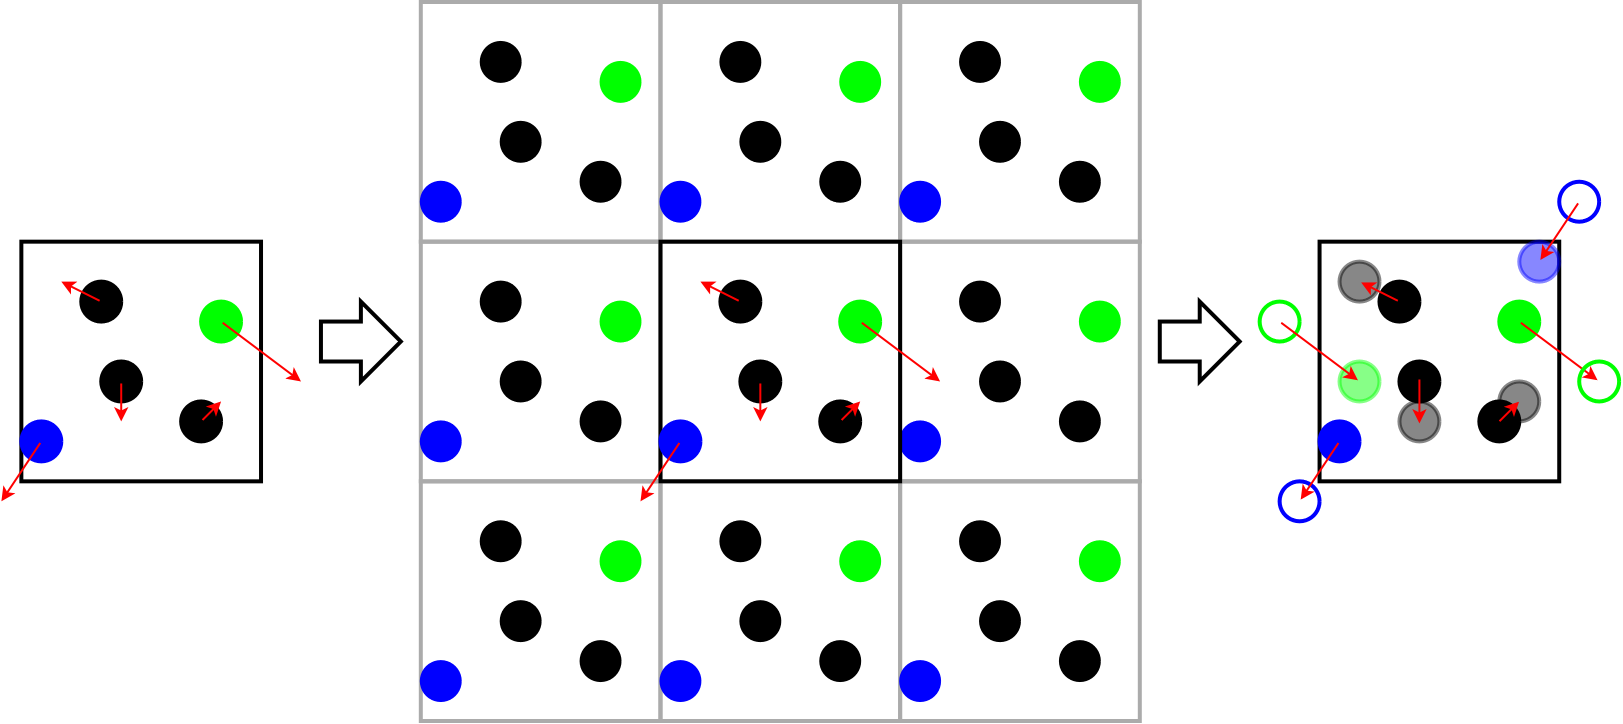
\includegraphics[width=0.6\linewidth]{../images/Boundary_Condition_explained_without_ghosts.png}
    \end{center}
\end{frame}

\begin{frame}{Project Description}{Particle interactions} 
    force computation of particle interactions:
    \begin{itemize}
        \tightlist
        \vspace*{-0.3\baselineskip}
        \item
          based on the Lennard-Jones potential:
          \begin{itemize}

              \tightlist
              \item pairs of particles, here: electronically neutral atoms
              \item models repulsive as well as attractive interactions
          \end{itemize}
    \end{itemize}
    \begin{center}
        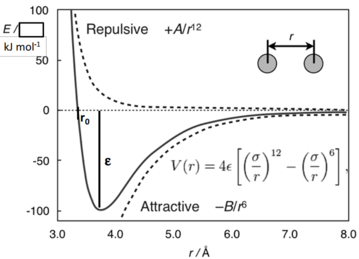
\includegraphics[width=0.35\textwidth]{../images/Lennard_Jones_potential_function.png}
    \end{center}
    
    
    \begin{itemize}
        \tightlist
        \item
          \emph{\textbf{r}} is the distance between the two interacting atoms,
        \item
          \emph{\textbf{ε}} is the dispersion energy and
        \item
          \emph{\textbf{σ}} the distance at which the particle-potential
          \emph{\textbf{V}} is zero
    \end{itemize}
\end{frame}

\begin{frame}[fragile]{Project Description}{Simulation Process}
    
    The simulation runs similar to the sketch code below:
    
    \begin{itemize}
        \tightlist
        \item every timestep iterate over all particles:
          \begin{itemize}
              \tightlist
              \item compute interactions with neighbors
              \item integrate force generated by interaction
          \end{itemize}
    \end{itemize}
    
    \begin{scriptsize}
    \begin{Shaded}
    \begin{Highlighting}[]
    \ControlFlowTok{for}\NormalTok{ t }\KeywordTok{in}\NormalTok{ timesteps:}
      \ControlFlowTok{for}\NormalTok{ atom }\KeywordTok{in}\NormalTok{ atoms:}
    \NormalTok{    velocity[atom] }\OperatorTok{+=}\NormalTok{ force[atom]}
    \NormalTok{    position[atom] }\OperatorTok{+=}\NormalTok{ velocity[atom]}
      \ControlFlowTok{if}\NormalTok{ t }\OperatorTok{%} \DecValTok{20} \OperatorTok{==} \DecValTok{0}\NormalTok{:}
    \NormalTok{    neighbors }\OperatorTok{=}\NormalTok{ calculateNeighbors()}
      \ControlFlowTok{for}\NormalTok{ atom }\KeywordTok{in}\NormalTok{ atoms:}
    \NormalTok{    neighbors }\OperatorTok{=}\NormalTok{ neighbors[atom]}
    \NormalTok{    force }\OperatorTok{=} \FloatTok{0.0}
        \ControlFlowTok{for}\NormalTok{ neighbor }\KeywordTok{in}\NormalTok{ neighbors:}
    \NormalTok{        radius }\OperatorTok{=}\NormalTok{ calc_radius(...)}
            \ControlFlowTok{if}\NormalTok{ radius }\OperatorTok{<}\NormalTok{ close_enough:}
    \NormalTok{            force }\OperatorTok{+=}\NormalTok{ calc_force(...)}
    \NormalTok{    forces[atom] }\OperatorTok{+=}\NormalTok{ force}
    \end{Highlighting}
    \end{Shaded}
    \end{scriptsize}
\end{frame}

\section{Testsystem}

\begin{frame}{Testsystem}    
    \begin{itemize}
        \tightlist
        \item Host/Clustername: alex
        \item multiple nodes with multiple GPUs per node
        \item
          resources per GPU:
        
          \begin{itemize}
          \tightlist
          \item
            {[}A40 \textbar{} A100{]}
          \item
            CPU: {[}16 cores / GPU \textbar{} 16 cores / GPU{]}
          \item
            Memory: {[}60GB / GPU \textbar{} 120GB / GPU{]}
          \end{itemize}
        \item computational power
        \begin{itemize}
            \item SP: {[}A40: 37.4 TFlops \textbar{} A100: 19.5 Tflops {]}
            \item DP: {[}A40: 0.5 TFlops \textbar{} A100: 9.7 Tflops {]}
        \end{itemize}
    \end{itemize}
    
    \textbf{Note}: each an A40 has about double the single precision
    processing power of an A100 despite being cheaper
\end{frame}

\section{Execution and default parameters}

\begin{frame}[fragile]{Executing the simulation}
    \begin{block}{Software Environment}
        \begin{itemize}
            \tightlist
            \item Compiler: NVCC (cuda/11.6.1)
            \item Operating System: Ubuntu 20.04.3 LTS
            \item Addition libraries:
            \begin{itemize}
                \tightlist
                \item LIKWID 5.2.0
            \end{itemize}
        \end{itemize}
    \end{block}
    
    \begin{block}{How to build software}
        \begin{verbatim}
$ git clone https://github.com/RRZE-HPC/MD-Bench/
$ cd MD-Bench
$ git checkout mucosim_cuda
$ module load likwid cuda
$ make
        \end{verbatim}
    \end{block}
    \vspace{-\baselineskip}
    \begin{block}{How to run software (e.g. in a batch job)}
        \begin{verbatim}
$ module load likwid cuda
$ cd MD-Bench
$ ./MDBench-NVCC
        \end{verbatim}
    \end{block}
\end{frame}

\begin{frame}[fragile]{Testcase description}
    \vspace*{-6\baselineskip}
    If not stated otherwise these are the conditions for the simulation benchmarking.
    
    \begin{itemize}
        \tightlist
        \item the number of simulated atoms is 131072
        \item floating point numbers use double precision
        \item force computation between atoms uses the lennard-jones model
        \item one gpu with its associated cores are used for computation
    \end{itemize}
\end{frame}

\section{First runtime tests}

\begin{frame}[fragile]{First runtime tests}{CPU Scaling runs}
    \vspace*{-6\baselineskip}
    \begin{itemize}
        \tightlist
        \item fixed: one gpu with its associated 16 cores
        \item scale the number of CPU-Threads
        \item take output of our programm contains line displaying throughput in number of atom updates per second:
    \end{itemize}
    
    \begin{verbatim}
    Performance: 7.18 million atom updates per second
    \end{verbatim}
\end{frame}

\begin{frame}[fragile]{First runtime tests}{CPU Scaling runs - continued}
    \begin{itemize}
        \item plot data for single- and double precision performance
    \end{itemize}
    \begin{center}
        
\includegraphics[width=0.5\linewidth]{../resources/initial_testing/linear_cpu-threads_scaling/SingleGPU_cpu_scaling.png}
    \end{center}

Similar convergence points in performance between the A40 and A100 hints at bottlenecks independent of the gpu.

\end{frame}

\section{Profiling the application}

\begin{frame}[fragile]{Profiling the application}{Using nsys}

		\begin{verbatim}
    srun nsys profile -o ./a40_profiling_run
		\end{verbatim}
    \begin{itemize}
    	\item to get this runtime timeline:
    \end{itemize}

    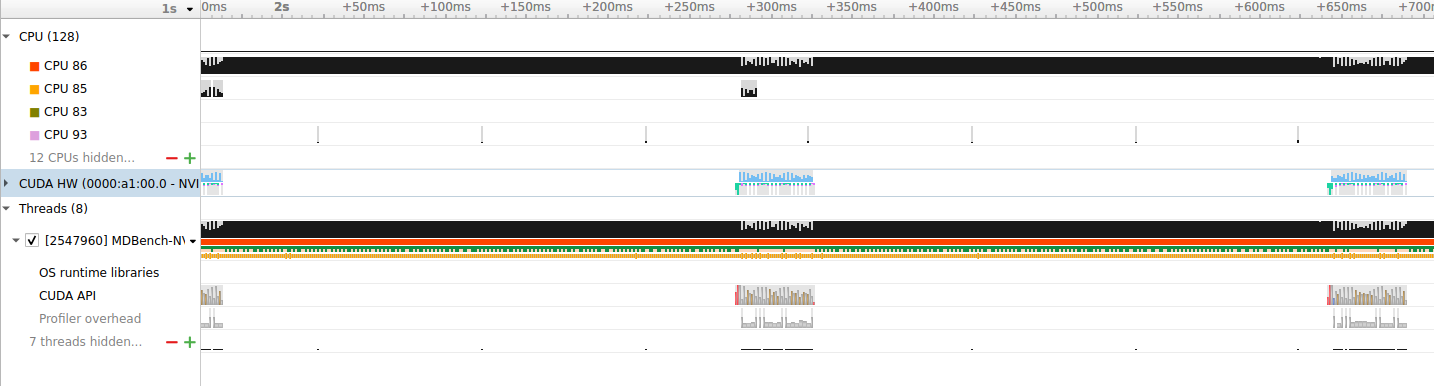
\includegraphics{../resources/initial_testing/finding_bottlenecks/using_nsys/A40_nsys_zoomed_in.png}

    \begin{itemize}
        \tightlist
        \item activity is cyclic
        \item most of the time is spent with only one CPU active
        \item short blue parts are where the GPU is active
    \end{itemize}
\end{frame}

\begin{frame}[fragile]{Profiling the application}{Finding where the CPU time is spent}
    \begin{itemize}
    	\item using \texttt{gprof}
    	\begin{itemize}
    		\item GPU time is not counted as such here
    	\end{itemize}
    \end{itemize}

    \begin{verbatim}
Flat profile:
Each sample counts as 0.01 seconds.
  %      self              total           
 time   seconds    calls  ms/call  name    
 97.70     3.35       11   306.47  buildNeighbor
  0.87     0.03      201     0.15  updatePbc
  0.58     0.02  2359296     0.00  myrandom
  0.58     0.02       11     1.82  binatoms
  0.29     0.01       11     0.91  setupPbc
  0.00     0.00     1668     0.00  checkCUDAError
  0.00     0.00      426     0.00  getTimeStamp
  0.00     0.00      201     0.00  computeForce
...
    \end{verbatim}
\end{frame}

\begin{frame}[fragile]{Profiling the application}{using runtime readings inside the program}
\vspace{-4\baselineskip}
    \begin{itemize}
    	\item in the standard program output
    	\begin{itemize}
    		\item tracks total time
    		\item takes both CPU and GPU into account
    		\item total runtime spent on the different phases
    	\end{itemize}
    \end{itemize}
    
    \begin{verbatim}
    TOTAL 3.47s FORCE 0.21s NEIGH 3.15s REST 0.12s
    \end{verbatim}
    
    Even when considering CPU and GPU time the neighbor calculation needs most of the time.
\end{frame}

\begin{frame}[fragile]{Profiling the application}{Explanation of runtime profile with program structure}

    Recall code from earlier:
    \begin{scriptsize}
        \begin{Shaded}
            \begin{Highlighting}[]
\ControlFlowTok{for}\NormalTok{ t }\KeywordTok{in}\NormalTok{ timesteps:}
    \ControlFlowTok{GPU-parallel-for}\NormalTok{ atom }\KeywordTok{in}\NormalTok{ atoms:}
    \NormalTok{    velocity[atom] }\OperatorTok{+=}\NormalTok{ force[atom]}
    \NormalTok{    position[atom] }\OperatorTok{+=}\NormalTok{ velocity[atom]}
    \ControlFlowTok{if}\NormalTok{ t }\OperatorTok{%} \DecValTok{20} \OperatorTok{==} \DecValTok{0}\NormalTok{:}
    \NormalTok{    neighbors }\OperatorTok{=}\NormalTok{ calculateNeighbors()}
    \ControlFlowTok{GPU-parallel-for}\NormalTok{ atom }\KeywordTok{in}\NormalTok{ atoms:}
    \NormalTok{    neighbors }\OperatorTok{=}\NormalTok{ neighbors[atom]}
    \NormalTok{    force }\OperatorTok{=} \FloatTok{0.0}
        \ControlFlowTok{for}\NormalTok{ neighbor }\KeywordTok{in}\NormalTok{ neighbors:}
    \NormalTok{        radius }\OperatorTok{=}\NormalTok{ calc_radius(...)}
            \ControlFlowTok{if}\NormalTok{ radius }\OperatorTok{<}\NormalTok{ close_enough:}
    \NormalTok{            force }\OperatorTok{+=}\NormalTok{ calc_force(...)}
                \NormalTok{forces[atom] }\OperatorTok{+=}\NormalTok{ force}
            \end{Highlighting}
        \end{Shaded}
    \end{scriptsize}
\end{frame}

\section{Parallelizing neighborhood calculation}

\begin{frame}[fragile]{Parallelizing neighborhood calculation}{neighborhood calculation process}
    \begin{itemize}
        \item real application simulates a 3D space
        \item examples written in pseudo-python assume a 2D space for simplicity and brevity
    \end{itemize}
        \vspace*{+.5\baselineskip}
    \begin{scriptsize}    
        \begin{Shaded}
            \begin{Highlighting}[]
\KeywordTok{def}\NormalTok{ calculate_neighbors():}
\NormalTok{  update_according_to(atoms, periodic_boundary_condition)}
\NormalTok{  setup_periodic_boundary_condition(atoms, periodic_boundary_condition)}
\NormalTok{  update_periodic_boundary_condition(atoms, periodic_boundary_condition)}
\NormalTok{  neighbor_list }\OperatorTok{=}\NormalTok{ build_neighbor(atoms)}
\ControlFlowTok{return}\NormalTok{ neighbor_list}
            \end{Highlighting}
        \end{Shaded}    
    \end{scriptsize}
    \begin{center}
        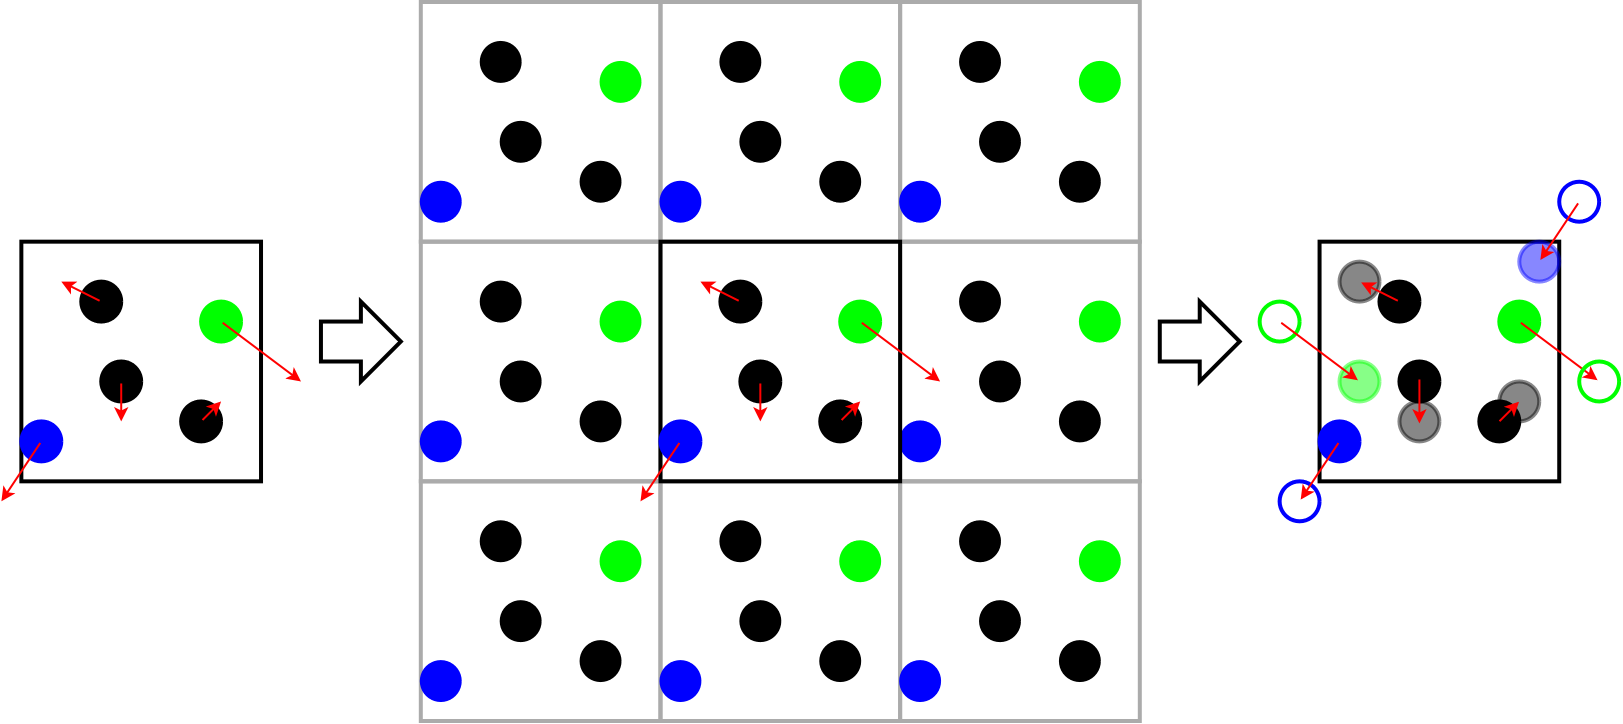
\includegraphics[width=0.4\linewidth]{../images/Boundary_Condition_explained_without_ghosts.png}
    \end{center}
\end{frame}

\begin{frame}[fragile]{Parallelizing neighborhood calculation}{Atom update}
    
    Atoms leaving the simulated area will enter on the mirrored side. In
    code it looks like this:
    \begin{scriptsize}
        \begin{Shaded}
            \begin{Highlighting}[]
\KeywordTok{def}\NormalTok{ update_according_to(atoms, periodic_boundary_condition):}
\NormalTok{  sim_width, sim_height }\OperatorTok{=}\NormalTok{ periodic_boundary_condition.simulated_area.dims}
\NormalTok{  x_max, x_min, y_max, y_min }\OperatorTok{=}\NormalTok{ periodic_boundary_condition.boundaries}
  \ControlFlowTok{for}\NormalTok{ atom }\KeywordTok{in}\NormalTok{ atoms:}
    \ControlFlowTok{if}\NormalTok{ position[atom].x }\OperatorTok{>}\NormalTok{ x_max:}
\NormalTok{      position[atom].x }\OperatorTok{-=}\NormalTok{ sim_width}
    \ControlFlowTok{if}\NormalTok{ position[atom].x }\OperatorTok{<}\NormalTok{ x_min:}
\NormalTok{      position[atom].x }\OperatorTok{+=}\NormalTok{ sim_width}
    \ControlFlowTok{if}\NormalTok{ position[atom].y }\OperatorTok{>}\NormalTok{ y_max:}
\NormalTok{      position[atom].y }\OperatorTok{-=}\NormalTok{ sim_height}
    \ControlFlowTok{if}\NormalTok{ position[atom].y }\OperatorTok{<}\NormalTok{ y_min:}
\NormalTok{      position[atom].y }\OperatorTok{+=}\NormalTok{ sim_height}
            \end{Highlighting}
        \end{Shaded}
    \end{scriptsize}

    \begin{itemize}
        \tightlist
        \item
          all iterations independent -\textgreater{} easy to parallelize
        \item one thread per atom for simplicity (GPU threads are quite lightweight)
    \end{itemize}
\end{frame}

\begin{frame}[fragile]{Parallelizing neighborhood calculation}{Ghost atoms for atoms near periodic border}
    
    Create ghost atoms on other side to emulate force interactions through
    the periodic border
    
    \begin{scriptsize}
        \begin{Shaded}
            \begin{Highlighting}[]
\KeywordTok{def}\NormalTok{ setup_periodic_boundary_condition(atoms, periodic_boundary_condition):}
\NormalTok{  ...}
\NormalTok{  n_ghosts }\OperatorTok{=} \DecValTok{0}\NormalTok{, }\NormalTok{  n_ghost_allocations }\OperatorTok{=}\NormalTok{ some_value}
\NormalTok{  ghosts }\OperatorTok{=}\NormalTok{ malloc(n_ghost_allocations }\OperatorTok{*}\NormalTok{ sizeof(ghost))}
  \ControlFlowTok{for}\NormalTok{ atom }\KeywordTok{in}\NormalTok{ atoms:}
    \ControlFlowTok{if}\NormalTok{ n_ghost_allocations }\OperatorTok{-}\NormalTok{ n_ghosts }\OperatorTok{<}\NormalTok{ max_ghosts_created_per_iteration:}
\NormalTok{      ghosts }\OperatorTok{=}\NormalTok{ reallocMore(ghosts, some_more)}
\NormalTok{      n_ghost_allocations }\OperatorTok{+=}\NormalTok{ some_more}
    \ControlFlowTok{if}\NormalTok{ position[atom].x }\OperatorTok{>}\NormalTok{ x_max }\OperatorTok{-}\NormalTok{ threshold:}
\NormalTok{      ghosts[n_ghosts}\OperatorTok{++}\NormalTok{] }\OperatorTok{=}\NormalTok{ createGhost(atom, }\OperatorTok{-}\NormalTok{sim_width, }\DecValTok{0}\NormalTok{)}
\NormalTok{    ...}
    \ControlFlowTok{if}\NormalTok{ position[atom].x }\OperatorTok{<}\NormalTok{ x_min }\OperatorTok{+}\NormalTok{ threshold AND position[atom] }\OperatorTok{<}\NormalTok{ y_min }\OperatorTok{+}\NormalTok{ threshold:}
\NormalTok{      ghosts[n_ghosts}\OperatorTok{++}\NormalTok{] }\OperatorTok{=}\NormalTok{ createGhost(atom, }\OperatorTok{+}\NormalTok{sim_width, }\OperatorTok{+}\NormalTok{sim_height)}
  
  \ControlFlowTok{if}\NormalTok{ n_atoms }\OperatorTok{+}\NormalTok{ n_ghosts }\OperatorTok{>} \BuiltInTok{len}\NormalTok{(atoms):}
\NormalTok{    atoms }\OperatorTok{=}\NormalTok{ realloc(n_atoms }\OperatorTok{+}\NormalTok{ n_ghosts)}
            \end{Highlighting}
        \end{Shaded}
    \end{scriptsize}
\end{frame}

\begin{frame}[fragile]{Parallelizing neighborhood calculation}{Updating the ghost atom positions}
    \vspace{-5\baselineskip}
    \begin{scriptsize}
    \begin{Shaded}
        \begin{Highlighting}[]
\KeywordTok{def}\NormalTok{ update_bondary_condition(atoms, periodic_boundary_condition):}
  \ControlFlowTok{for}\NormalTok{ ghost }\KeywordTok{in}\NormalTok{ ghosts:}
\NormalTok{    position[ghost].x }\OperatorTok{=}\NormalTok{ ghost.offset_x }\OperatorTok{+}\NormalTok{ position[ghost.original].x}
\NormalTok{    position[ghost].y }\OperatorTok{=}\NormalTok{ ghost.offset_y }\OperatorTok{+}\NormalTok{ position[ghost.original].y}
        \end{Highlighting}
    \end{Shaded}
    \end{scriptsize}
    \begin{itemize}
        \tightlist
        \item iterations independent
        \begin{itemize}
            \tightlist
            \item easy to parallelize -\textgreater{} one thread per atom
        \end{itemize}
    \end{itemize}
\end{frame}

\begin{frame}[fragile]{Parallelizing neighborhood calculation}{Building neighbor lists}
    \begin{scriptsize}
        \begin{Shaded}
            \begin{Highlighting}[]
\KeywordTok{def}\NormalTok{ buildNeighbor(atoms):}
\NormalTok{  ...}
\NormalTok{  grid_cells }\OperatorTok{=}\NormalTok{ sort_into(atoms), } \NormalTok{  neighbor_list }\OperatorTok{=}\NormalTok{ malloc(...)}
\NormalTok{  resize_needed }\OperatorTok{=}\NormalTok{ true}
  \ConstantTok{do:}
\NormalTok{    new_max_neighbors_per_atom }\OperatorTok{=}\NormalTok{ max_neighbors_per_atom}
\NormalTok{    resize_needed }\OperatorTok{=}\NormalTok{ false}
    \ControlFlowTok{for}\NormalTok{ atom }\KeywordTok{in}\NormalTok{ atoms:}
\NormalTok{      neighbor_count }\OperatorTok{=} \DecValTok{0}\NormalTok{,    grid_cell }\OperatorTok{=}\NormalTok{ grid_cell_of(position[atom])}
      \ControlFlowTok{for}\NormalTok{ other_atom }\KeywordTok{in}\NormalTok{ (neighboring_cells(grid_cell) + grid_cell).atoms:}
        \ControlFlowTok{if}\NormalTok{ other_atom == atom: continue}
        \ControlFlowTok{if}\NormalTok{ distance(atom, other_atom) }\OperatorTok{<}\NormalTok{ threshold:}
\NormalTok{          neighbor_list[atom,}\NormalTok{ neighbor_count++] }\OperatorTok{=}\NormalTok{ other_atom}
      \ControlFlowTok{if}\NormalTok{ neighbor_count }\OperatorTok{>}\NormalTok{ max_neighbors_per_atom:}
\NormalTok{        resize_needed }\OperatorTok{=}\NormalTok{ true}
        \ControlFlowTok{if}\NormalTok{ neighbor_count }\OperatorTok{>}\NormalTok{ new_max_neighbor_count_per_atom:}
\NormalTok{          new_max_neighbor_count_per_atom }\OperatorTok{=}\NormalTok{ neighbor_count}
    \ControlFlowTok{if}\NormalTok{ resize_needed:}
\NormalTok{      max_neighbors_per_atom }\OperatorTok{=}\NormalTok{ new_max_neighbors_per_atom }\OperatorTok{*} \FloatTok{1.2}
\NormalTok{      free(neighbor_list),}\NormalTok{      neighbor_list }\OperatorTok{=}\NormalTok{ malloc(...)}
  \ControlFlowTok{while}\NormalTok{(resize_needed)}
            \end{Highlighting}
        \end{Shaded}
    \end{scriptsize}
\end{frame}

\begin{frame}{Next goals}
    \vspace{-3\baselineskip}
    \begin{itemize}
        \item port the buildNeighbor-function to Cuda
    \begin{itemize}
        \item reduces Host-To-Device traffic
        \item reduces computation time
    \end{itemize}
    \item port function updating the ghost atoms to Cuda
    \item port creating the ghost atoms to Cuda
    
    \vspace{\baselineskip}
    \item evaluate performance along the way
    \end{itemize}


\end{frame}

\begin{frame}
    \begin{center}
        \color{blue}
        \begin{Huge}
        Thank you 
        
        for your attention
    \end{Huge}
    \vspace{\baselineskip}

    \color{black}
    \begin{LARGE}
        Any questions?
    \end{LARGE}

    \begin{large}
        Any other ideas for parallelization?
    \end{large}
    \end{center}


\end{frame}

\end{document}
